\section{Optimizing Linear Transformations}
As we will show in Chapter \ref{chp:inverseImpl}, the isomorphism functions and their inverses can be seen as binary matrix multiplications. Therefore, it is natural to attempt to optimize these matrix multiplications by reducing the total number of XOR gates required in a combinational implementation. Formally, this problem is known as the \emph{Shortest Linear Program} (SLP) problem. We borrow the notation of \cite{Boyar08-1} to describe it in sufficient detail. Let $\mathbb{F}$ be a field and let $E$ be a set of $m$ linear forms over the field $\mathbb{F}$, similar to those shown below.
\begin{gather*}
\alpha_{1,1}x_1 + \alpha_{1,2}x_2 + \dots + \alpha_{1,n} \\
\alpha_{2,1}x_1 + \alpha_{2,2}x_2 + \dots + \alpha_{2,n} \\
\dots \\
\alpha_{m,1}x_1 + \alpha_{m,2}x_2 + \dots + \alpha_{m,n},
\end{gather*}
where $\alpha_{i,j} \in \mathbb{F}$, $1 \leq i \leq m$, $1 \leq j \leq n$, and $x_{i}$, $1 \leq i \leq n$, are variables over $\mathbb{F}$. For later reference, note that it is often convenient to store the coefficients $\alpha_{i,j}$ in an $m\times n$ matrix $\mathbf{A}$ over $GF(2)$. We can model this computation as a \emph{linear straight-line program}, in which each line of the program is of the form $u := \lambda v  + \mu w$, where $\lambda$ and $\mu$ are elements in $\mathbb{F}$ and $u$, $v$, and $w$ are variables, and some lines map directly to the output of the corresponding linear form. Linear straight line programs are also constrained in that \emph{variables} cannot be multiplied together. An optimal linear straight line program is the shortest such linear program that computes a set of linear forms, where the length of the program is measured in terms of the number of lines. If we consider linear forms over $GF(2)$, then minimal straight line linear programs correspond to the smallest linear circuit consisting of only XOR gates that compute the same set of linear forms. 

A linear straight line program over $GF(2)$ is said to be cancellation free if and only if for every line $u := v + w$, the expressions for $v$ and $w$ do not contain any shared variables. For example, if $v = x_1 + x_2$ and $w = x_1 + x_3$, then $u = v + w + (x_1 + x_2) + (x_1 + x_3) = x_2 + x_3$ after cancellation. If the $x_1$ variables were factored out of the expressions for $v$ and $w$, then we would obtain a shorter, possibly \emph{cancellation-free} program. However, this process of factorization does not always yield optimal linear straight line programs. To show this, consider the following set of linear forms:
\begin{align*}
y_0 & := x_1 + x_2 \\
y_1 & := x_1 + x_2 + x_3 \\
y_2 & := x_1 + x_2 + x_3 + x_4 \\
y_3 & := x_2 + x_3 + x_4 
\end{align*}
The equivalent optimal cancellation-free program for computing this linear form is as follows:
\begin{align*}
u_1 & := x_1 + x_2 \: (y_0)\\
u_2 & := u_1 + x_3 \: (y_1)\\
u_3 & := u_2 + x_4 \: (y_2)\\
v_1 & := x_2 + x_3 \\
u_4 & := v_1 + x_4 \: (y_3)
\end{align*}
However, if we allow cancellation, we may compute this same program in only four lines:
\begin{align*}
u_1 & := x_1 + x_2 \: (y_0)\\
u_2 & := u_1 + x_3 \: (y_1)\\
u_3 & := u_2 + x_4 \: (y_2)\\
u_4 & := u_3 + x_1 \: (y_3)
\end{align*}
Obtaining the optimal straight line linear program (represented as a linear circuit) for a particular set of linear forms is an NP-hard problem; there exists a polynomial time reduction from VERTEX-COVER \cite{Boyar08-1}, one of Karp's $21$ NP-COMPLETE problems \cite{Karp72-1}. Boyar and Peralta also showed that techniques for producing optimal cancellation-free straight line programs has an approximation ratio of at least $3/2$ \cite{Boyar08-1}, making the most approximation techniques for optimizing sets of linear forms with $16$ equations (i.e. those used for $16 \times 16$ binary matrix multiplications) far from optimal. 

\subsection{Heuristic-Based Optimizations} \label{sec:linearOptTechniques}
The majority of the work focused on trying to find optimal straight line linear programs is based on greedy algorithms flavored with decision heuristics. To date, some of the most effective heuristics are those based on the greedy factorization technique presented by Paar \cite{Paar97-1}. The algorithm is quite simple and works as follows. At each iteration the pair of distinct variables $x_i + x_j$ that occurs most frequently among the set of linear forms is determined. Then, a new variable $x_{\mu} = x_i + x_j$ is introduced and substituted into all linear forms that contained the pair $x_i + x_j$. During the next iteration of the algorithm, the new variable $x_{\mu}$ is considered when selecting the new most frequently occurring pair, and the variable selection and substitution process repeats. The algorithm terminates when there are no pairs of variables that are shared across more than one form. Algorithm \ref{alg:greedyMatrixOptimizePaar} gives a complete description of this procedure. As indicated by Paar, the greedy nature of this algorithm means that it only achieves a locally optimal solution; it is not globally optimal. However, he does not a modification to the algorithm that can improve the results, where instead of considering a single pair of variables that is shared with the highest frequency among all linear forms, one considers \emph{all} pairs of variables that occur with the highest frequency.

\begin{algorithm}[ht!] %[htb]
\caption{Greedy linear form optimization \cite{Paar97-1}} \label{alg:greedyMatrixOptimizePaar}
\begin{algorithmic}[1]
	\Require A binary matrix $\mathbf{A}$ representing a set of linear forms, where each linear form has length $n$
	\State $m \gets n - 1$
	\State $\mathbf{M} \gets \mathbf{A}$
	\State $hmax \gets 0$
	\State $maxi \gets 0$
	\State $maxj \gets 0$
	\Repeat 
		\For{$i = 0 \to m - 1$}
			\For{$j = 0 \to m$}
				\State $coli \gets $GETCOLUMN$(\mathbf{M}, i)$
				\State $colj \gets $GETCOLUMN$(\mathbf{M}, j)$
				\If{HW$(coli $ \& $ colj) > hmax)$}
					\State $hmax \gets $HW$(coli $ \& $ colj)$
					\State $maxi \gets coli$
					\State $maxj \gets colj$
				\EndIf
			\EndFor
		\EndFor
		\If {$hmax > 1$}
			\State $maxcoli \gets $GETCOLUMN$(\mathbf{M}, maxi)$
			\State $maxcolj \gets $GETCOLUMN$(\mathbf{M}, maxj)$
			\State $newcol \gets maxcoli $ \& $ maxcolj$
			\State PUTCOLUMN$(\mathbf{M}, newcol, m + 1)$
			\State PUTCOLUMN$(\mathbf{M}, $NEGATE$(newcol $ \& $ maxcoli), maxi)$
			\State PUTCOLUMN$(\mathbf{M}, $NEGATE$(newcol $ \& $ maxcolj), maxj)$
			\State $m \gets m + 1$
		\EndIf
	\Until{$hmax \leq 1$}
	\State \Return $\mathbf{M}$
\end{algorithmic}
\end{algorithm}

For $16 \times 16$ matrices, Paar's algorithm was shown to provide an improvement (in terms of the number of XOR gates required) of approximately $47.2\%$. As an example of this algorithm, consider the following set of linear forms:
\begin{align*}
y_0 & := x_0 + x_1 + x_2 \\
y_1 & := x_1 + x_3 + x_4 \\
y_2 & := x_0 + x_2 + x_3 + x_4 \\
y_3 & := x_1 + x_2 + x_3 \\
y_4 & := x_0 + x_1 + x_3 \\
y_5 & := x_1 + x_2 + x_3 + x_4
\end{align*}

We may represent this set of linear forms with the binary matrix $\mathbf{A}$ as follows:
\begin{align*} 
\mathbf{A} = 
\begin{pmatrix}
1 & 1 & 1 & 0 & 0 \\
0 & 1 & 0 & 1 & 1 \\
1 & 0 & 1 & 1 & 1 \\
0 & 1 & 1 & 1 & 0 \\
1 & 1 & 0 & 1 & 0 \\
0 & 1 & 1 & 1 & 1
\end{pmatrix}
\end{align*}
This can then be computed using a linear circuit with $8$ XOR gates. However, upon careful inspection it is clear that there exists many redundancies in this circuit (e.g. the sum $x_1 + x_2$ is computed more than once). If we remove all such redundant computations through greedy factorization, we find an equivalent linear circuit with a smaller gate count shown below in matrix form.
\begin{align*} 
\mathbf{A} = 
\begin{pmatrix}
0 & 1 & 0 & 0 & 0 & 0 & 1 & 0 \\
0 & 0 & 0 & 0 & 1 & 1 & 0 & 0 \\
0 & 0 & 0 & 1 & 1 & 0 & 1 & 0 \\
0 & 0 & 0 & 0 & 0 & 0 & 0 & 1 \\
1 & 0 & 0 & 0 & 0 & 1 & 0 & 0 \\
0 & 0 & 0 & 0 & 1 & 0 & 0 & 1 \\
\end{pmatrix}
\end{align*}

% \begin{figure}[ht]
% \centering
% \subfigure[Unoptimized linear circuit.]{
%     % \rule{2cm}{3cm}
%     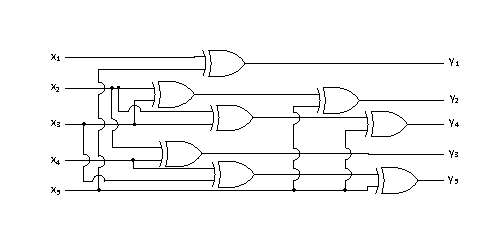
\includegraphics[scale=0.8]{./chapter_optimize/cse.pdf}
%     \label{fig:linearCircuita}
% }
% \subfigure[Equivalent cancellation-free linear circuit]{
%     % \rule{2cm}{3cm}
%     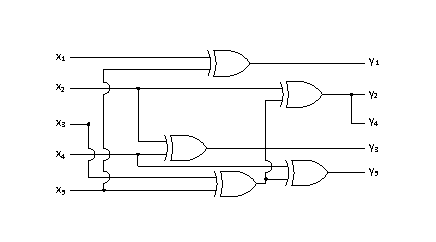
\includegraphics[scale=0.8]{./chapter_optimize/cse_opt.pdf}
%     \label{fig:linearCircuitb}
% }
% \caption{Two linear circuits that compute the same function. The left circuit is unoptimized and the right circuit is fully factored (cancellation-free).}
% \end{figure}

In 2009, Daniel Bernstein \cite{Bernstein09-1} published another algorithm for optimizing software implementations of linear maps modulo $2$ (i.e. linear forms with coefficients in $\mathbb{F}_2$). The main idea of this algorithm is as follows: given the linear forms $L_0,L_1,\dots,L_{q-1}$, input vector $x$ and output vector $y$, both of length $q$, compute the $q$ dot products $L_0 \cdot x$, $L_1 \cdot x$, \dots, $L_{q-1} \cdot x$, where $L_0 \geq L_1 \geq \dotsb \geq L_{q-1}$ and store the results in the coordinates of $y$. Motivated by the Bos-Coster approach \cite{Rooji95-1}, the algorithm recursively computes $(L_0 - L_1) \cdot x, L_1\cdot x,\dots, L_{q-1}$ and then adds $y_1$ into $y_0$ (i.e. $y_0 + y_1 = L_0 - L_1 + L_1 = L_0$). A modified description of the algorithm is given in Algorithm \ref{alg:bernsteinLinearOpt}.

\begin{algorithm}[ht!] %[htb]
\caption{Bernstein recursive optimization (transcribed from \cite{Bernstein09-1})} \label{alg:bernsteinLinearOpt}
\begin{algorithmic}[1]
	\Require $q$ Linear forms $L_0,L_1,\dots,L_{q-1}$, each of length $p$, and input and output vectors $x$ and $y$ such that $|x| = |y| = q$
	\If {$q = 0$}
		\State Stop.
	\EndIf
	\If {$p = 0$}
		\State Generate code that sets $y_i = 0$ for all $0 \leq i \leq q-1$.
		\State Stop.
	\EndIf
	\State Find $j \in \{0,1,\dots,q-1\}$ that maximizes $L_j$ in reverse lexicographical order.
	\If {$L_j[p-1] = 0$}
		\State Recurse with $L_k' = (L_k[0],\dots,L_k[p-2])$ for each $k = 0,1,\dots,q-1$.
		\State Stop.
	\EndIf
	\If {$q \geq 2$}
		\State Find $i \in \{0,1,\dots,q-1\} \setminus \{j\}$ that maximizes $L_i$ in reverse lexicographical order.
		\If {$L_i[p-1] = 1$}
			\State Recurse with $L_k' = L_k$ for all $k \in \{0,1,\dots,q-1\}$ and $L_j' = L_j \oplus L_i$, and ``insert'' one
			XOR gate that adds $x_i$ and $x_j$ and stores the result in $x_j$.
			\State Stop.
		\EndIf
		\State Recurse with $L_k' = L_k$ for each $k = 0,1,\dots,q-1$ except that $L_j'[p-1] = 0$, and ``insert'' one
		XOR gate that adds $x_{p-1}$ into output bit $y_j$.
		\State Stop.
	\EndIf
\end{algorithmic}
\end{algorithm}

For $16 \times 16$ matrices, Bernstein reported that the average cost after zero elimination, divided by $16 \times 16 = 256$, was $0.2694$, meaning that the average cost for a $16 \times 16$ matrix multiplication over $GF(2)$ was $16 \times 16 \times 0.2694 = 68.9664$ XOR gates, which is more than the reported $59.1$ average from Paar's technique. In general, our experiments confirm that, on average, Bernstein's technique yields linear programs with a larger number of gates than Paar's greedy factorization technique. 

Boyar and Peralta \cite{Boyar12-1} introduced another heuristic in 2012, which appears to offer the best results since Paar's technique. At a high level, the algorithm greedily searches for the smallest linear circuit that is equivalent to the input set of linear forms by building new linear combinations of functions from a set of ``known'' functions. More formally, the algorithm works by continually decreasing the distance $\delta(S, f)$, which is the minimum number of additions from functions in $S$ necessary to obtain the predicate $f$, for each $f_0,\dots,f_{n-1}$, where $f_0,\dots,f_{n-1}$ are the $n$ linear forms being optimized. The original ``base'' of $S$ consists of the functions corresponding to the predicate variables $x_0,\dots,x_{n-1}$. The algorithm iterates while the $\delta(S, f_i) \not= 0$ for all $0 \leq i \leq n-1$, and at each iteration adds a new base function $S_{\mu} = S_i + S_j$ for some pair of base functions $S_i$ and $S_j$ to $S$, updates the distances $\delta(S, f_i)$ for all $0 \leq i \leq n - 1$, and then repeats. The selection of $S_i$ and $S_j$ is made such that the new distances are minimized, where ties are handled according to one of the following rules:
\begin{enumerate}
	\item Maximize the Euclidean norm of the vector of distances.
	\item Maximize the square of the Euclidean norm minus the largest distance.
	\item Maximize the square of the Euclidean norm minus the difference of the largest two distances.
	\item With probability $p = 0.5$ select the first possible base pairs out of the set of possibilities, and with probability
	$1 - p = 0.5$ apply the Euclidean norm rule and choose the largest one.
\end{enumerate}

In cases where optimal linear programs are needed, these heuristic-based approximations are not always effective. Fuhs and Schneider-Kamp \cite{Fuhs10-1} were able to cleverly encode a linear program of length $k$ for set of linear forms $f_1,\dots,f_m$ into first order propositional logic. If a satisfiable model for the equivalent Boolean formula $\phi$ exists, then the shortest linear program is easily reconstructed from the model. Otherwise, there does not exist a straight line linear program of length $k$ that computes the $m$ linear forms. 

For a system of $m$ linear forms with input coefficients represented with a binary matrix $\mathbf{A}$, the optimal length $k^*$ of an equivalent straight line linear program lies in the closed interval $[m, |\mathbf{A}|_1 - m - 1]$. Using this fact and the provably correct method to determine if a linear program of length $k$ exists for a particular set of linear forms, the authors then search for the optimal solution by iteratively applying the SAT solver technique for consecutive values of $k$ in decreasing order until an unsatisfiable instance is found. Once this limit is reached, the optimal value of $k^*$ must be then $k + 1$.

This technique was tested on the upper and lower linear transformations that make Boyar and Peralta's area-efficient S-box. It was able to verify their $k^* = 23$ linear program length presented in \cite{Boyar12-1}. While, the $k = 20$ case is trivially shown to be unsatisfiable due to the pigeonhole principle, the SAT instance for $k \in \{21, 22\}$ proved to be too difficult for modern SAT solvers to solve, even with various preprocessing and tuning techniques presented in the paper. Since replicating this work and implementing this procedure is nontrivial, we leave the experimentation with this technique on the matrix candidates in this work to future work. 

\subsection{Improving Linear Circuit Minimization Efficiency}
We implemented the previously discussed algorithms in our circuit optimization library and tested the results of each one for $16 \times 16$ and $32 \times 16$ matrices, which are of interest in this work. Our results, which are summarized in Table \ref{tab:algComparison}, clearly show that the Boyar-Peralta heuristic optimization technique yields the smallest values for all cases with little difference between the four different tie breaking rules. 
\begin{table}
\caption{Comparison of different optimization algorithms for the target $16 \times 16$ and $32 \times 16$ matrices in this work. The average XOR counts were gathered by populating the entries of matrices with nonzero entries with probability $p = 0.5$ over a series of $500$ trials.}
\label{tab:algComparison}
\begin{center}
	\begin{tabular}{| c | c | c |} \hline
		\emph{Matrix Size} & \emph{Algorithm} & \emph{Average XOR Count} \\ \hline
		$16 \times 16$ & Paar Factorization & 58.14 \\
		$16 \times 16$ & Boyar-Peralta Optimization \#1 & 50.09 \\
		$16 \times 16$ & Boyar-Peralta Optimization \#2 & 50.11 \\
		$16 \times 16$ & Boyar-Peralta Optimization \#3 & 50.09 \\
		$16 \times 16$ & Boyar-Peralta Optimization \#4 & 53.1 \\
		$16 \times 16$ & Bernstein Optimization & 85.0 \\ \hline
		$32 \times 16$ & Paar Factorization & 103.89 \\
		$32 \times 16$ & Boyar-Peralta Optimization \#1 & 83.22 \\
		$32 \times 16$ & Boyar-Peralta Optimization \#2 & 83.27 \\
		$32 \times 16$ & Boyar-Peralta Optimization \#3 & 83.22 \\
		$32 \times 16$ & Boyar-Peralta Optimization \#4 & 88.15 \\
		$32 \times 16$ & Bernstein Optimization & 146.66 \\ \hline
	\end{tabular}
\end{center}
\end{table}

While these heuristic-based optimization techniques may come close to optimal solutions, doing so is not guaranteed. In the context of cryptographic applications, Canright was the first to utilize an exhaustive, tree-based search for optimal cancellation-free linear programs \cite{Canright05-1}. The algorithm works by recursively inserting a new variable $x_{\mu} = x_i + x_j$ for all pairs of variables $x_i$ and $x_j$ that are shared by more than one linear form and returning the selection that yields the smallest number of gates. We give a complete description of the procedure in Algorithm \ref{alg:exhaustiveCanright}. Due to the combinatorial complexity of the algorithm, it is difficult to quantify its exact running time. 

\begin{algorithm}[ht!] %[htb]
\caption{SequentialExhaustiveFactor($M$, $m$, $g$)} \label{alg:exhaustiveCanright}
\begin{algorithmic}[1]
	\State $g' \gets g$
	\For{$i = 0 \to m - 1$}
		\For{$j = 0 \to m$}
			\State $coli \gets $GETCOLUMN$(M, i)$
			\State $colj \gets $GETCOLUMN$(M, j)$
			\If{HW$(coli $ \& $ colj) > 1)$}
				\State $M' \gets COPY(M)$
				\State $newcol \gets maxcoli $ \& $ maxcolj$
				\State $wt \gets $HW($newcol)$
				\State PUTCOLUMN$(M', newcol, m + 1)$
				\State PUTCOLUMN$(M', $NEGATE$(newcol $ \& $ maxcoli), maxi)$
				\State PUTCOLUMN$(M', $NEGATE$(newcol $ \& $ maxcolj), maxj)$
				\State $gc \gets $SequentialExhaustiveFactor$(M', m+1, g - wt + 1)$
				\If {$gc < g'$}
					\State $g' \gets gc$
				\EndIf
			\EndIf
		\EndFor
	\EndFor
	\State \Return $g'$ 
\end{algorithmic}
\end{algorithm}

The only optimizations applied to this algorithm were elementary pruning techniques to avoid redundant tree branches. To our knowledge, no one has explored parallel implementations of this algorithm. Therefore, this is a fruitful opportunity to increase the dimension of matrices which can be fully optimized, thereby aiding our optimization step for $16 \times 16$ matrices. The parallel implementation of the algorithm, written in Java, makes use of the fork/join parallel programming pattern to perform a breadth first traversal of the matrix factorization tree. The algorithm is driven by a collection of worker threads which retrieve matrices from a pool of those discovered during the breadth-first traversal of the tree. The worker threads are managed by the Java ForkJoinPool service which execute an {\tt optimize()} method in a class entitled ParallelMatrixOptimize. A thorough snippet of the source code for the parallel factorization program is shown in Appendix \ref{app:sourceCode}, and the pseudocode description of the entire parallel algorithm is presented in Algorithm \ref{alg:parallelOptimize}.

\begin{algorithm}[ht!] %[htb]
\caption{ParallelExhaustiveFactor($M$, $m$, $g$)} \label{alg:parallelOptimize}
\begin{algorithmic}[1]
	\State $g' \gets g$
	\State $P \gets []$
	\For{$i = 0 \to m - 1$}
		\For{$j = 0 \to m$}
			\State $coli \gets $GETCOLUMN$(M, i)$
			\State $colj \gets $GETCOLUMN$(M, j)$
			\If{HW$(coli $ \& $ colj) > 1)$}
				\State $P \gets Append(P, (i, j))$
			\EndIf
		\EndFor
	\EndFor
	\State $T \gets []$
	\For{$(i, j) \in P$}
		\State $M' \gets COPY(M)$
		\State $newcol \gets maxcoli $ \& $ maxcolj$
		\State $wt \gets $HW($newcol)$
		\State PUTCOLUMN$(M', newcol, m + 1)$
		\State PUTCOLUMN$(M', $NEGATE$(newcol $ \& $ maxcoli), maxi)$
		\State PUTCOLUMN$(M', $NEGATE$(newcol $ \& $ maxcolj), maxj)$
		\State $T \gets Append(T, (M', m + 1, g - wt + 1))$
	\EndFor
	\State $R \gets invokeAll(ParallelExhaustiveFactor(T))$
	\For {$r \in R$}
		\If {$r.gc < g'$}
			\State $g' \gets r.gc$
		\EndIf
	\EndFor
	\State \Return $g'$ 
\end{algorithmic}
\end{algorithm}

We present a comparison of the performance against the Canright's sequential version (translated from his C program to Java) and our parallel factorization algorithm in Table \ref{tab:factorTimes}. On average, factoring matrices larger than $10 \times 10$ and $14 \times 7$ took an unreasonable amount of time to finish for the purpose of this experiment, as insinuated by Canright \cite{Canright05-1}. This led us to not pursue any further techniques for optimizing this particular algorithm. As a result, an exhaustive factorization for $16 \times 16$ and $32 \times 16$ matrices, which are the focus in this work, needed to be done with different and more efficient optimization techniques.

\begin{table}
\label{tab:factorTimes}
\caption{Comparison of the factorization time using the sequential and parallel factorization programs. }
\begin{center}
	\begin{tabular}{| c | c | c |} \hline
	$m \times n$ & \emph{Sequential Time (msec)} & \emph{Parallel Time (msec)} \\ \hline
	$7 \times 7$ & 16 & 15 \\ 
	$8 \times 8$ & 16 & 17 \\ 
	$9 \times 9$ & 188 & 79 \\ 
	$10 \times 10$ & 4625 & 1703 \\ 
	$12 \times 6$ & 9 & 9 \\
	$14 \times 7$ & 247 & 93 \\ \hline
	\end{tabular}
\end{center}
\end{table}

In addition to parallelizing the exhaustive factoring algorithm, we also implemented a parallel version of Boyar and Peralta's technique using the Parallel Java library \cite{Kaminsky10-1}. During the course of our preliminary experiments we observed that the computation of $\delta(S, f)$ was responsible for a large portion of program's overall execution time. Therefore, to speed up this computation, our parallel version of this technique evenly distributes and performs computation of $\delta(S, f)$ using multiple threads on an shared-memory multiprocessor (SMP) machine, thus enabling faster speedups as the dimension of the input set of linear forms increases (small sets of linear forms suffer from overhead of the parallel computing framework - i.e. thread team configuration and synchronization). See Appendix \ref{app:sourceCode} for a snippet of the source code for this program.

To study the performance gains of the parallel equivalents of this algorithm, we first denote the input problem size $N$ as the number of elements in the matrix representing the linear forms, $T$ as the execution time for a particular program run, and $K$ as the number of processors available for computation. We define sizeup as the ratio of the problem size solved for a given execution time to the number of processors available for computation, captured below as
\begin{align*}
Sizeup(T,K) = N_{par}(T,K) / N_{seq}(T,1)
\end{align*}
Similarly, we define speedup as the ratio of the problem execution time for a given problem size to the number of processors available for computation, captured below as
\begin{align*}
Speedup(N, K) = T_{seq}(N, K) / T_{par}(N, K)
\end{align*}
Since both sizeup and speedup are important when scaling up to $16 \times 16$ and $32 \times 16$ matrices, we measured each for $K = 1$, $2$, $3$, $4$, and $8$ processors to see how the parallel implementations scaled and approached the limit imposed by Amdahl's law. The results from these experiments for the first tie breaker in Boyar and Peralta's technique on an eight-processor SMP machine with with four UltraSPARC-IV dual-core processors, a 1.35 GHz clock frequency, and 16 GB of main memory are shown in Figures \ref{fig:speedup1}, \ref{fig:speedup2}, \ref{fig:sizeup1} and \ref{fig:sizeup2}. Notice that, although we appear to achieve efficient speedups limited by Amdahl's law, our the parallel implementations do not achieve efficient sizeups. This is an indication that running these programs on larger problems may not yield improved running times. Even still, our results show significant improvements for the $16 \times 16$ and $32 \times 16$ matrices that are the focus of this work, thus enabling us to process many more linear programs in a shorter amount of time. As a result, these parallel implementations should prove useful for related research. 

\begin{figure}
\begin{center}
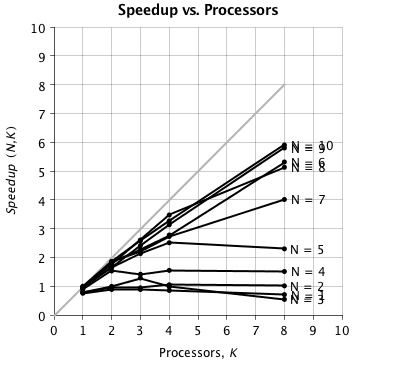
\includegraphics[scale=0.35]{./chapter_optimize/t1u_speed_3.png}
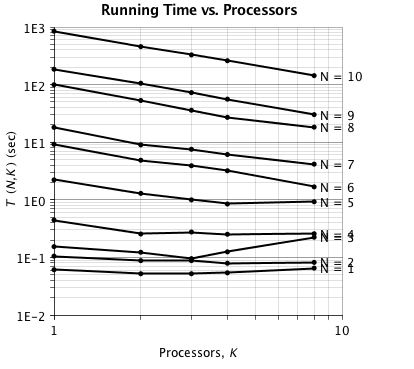
\includegraphics[scale=0.35]{./chapter_optimize/t1u_speed_4.png}
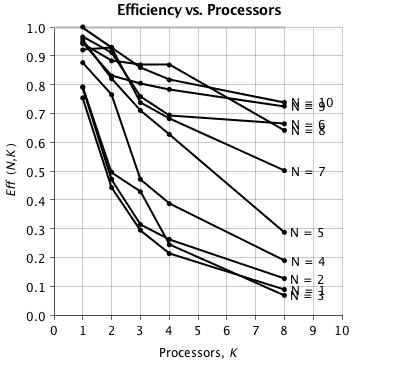
\includegraphics[scale=0.35]{./chapter_optimize/t1u_speed_2.png}
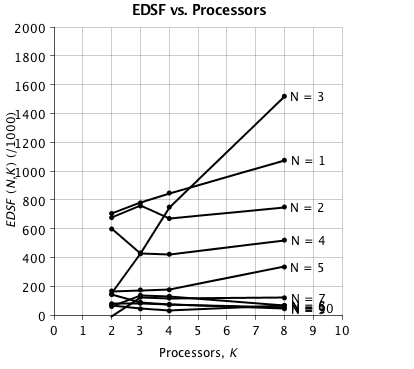
\includegraphics[scale=0.35]{./chapter_optimize/t1u_speed_1.png}
\caption{Speedup metrics for the parallel implementation of Boyar and Peralta's technique using tie breaker \#1 with $16 \times 16$ matrices. In these graphs we use $N = 1$ to denote $7 \times 7$ matrices, $N = 2$ to denote $8 \times 8$ matrices, etc.}
\label{fig:speedup1}
\end{center}

\begin{center}
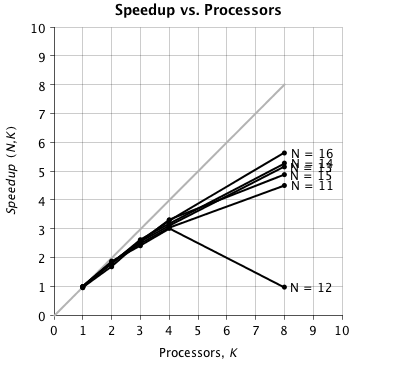
\includegraphics[scale=0.35]{./chapter_optimize/t1m_4.png}
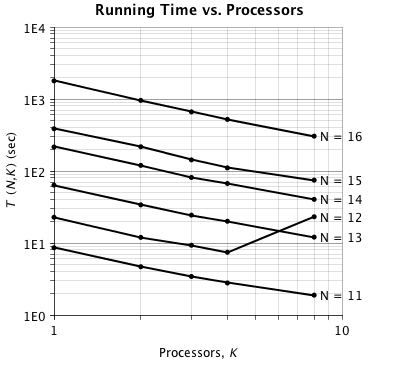
\includegraphics[scale=0.35]{./chapter_optimize/t1m_1.png}
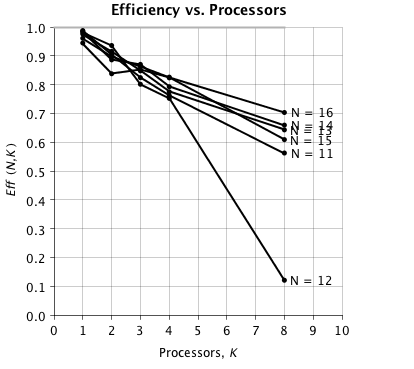
\includegraphics[scale=0.35]{./chapter_optimize/t1m_3.png}
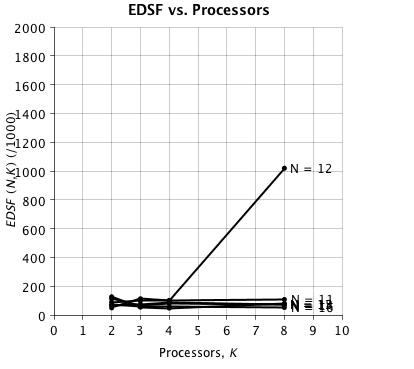
\includegraphics[scale=0.35]{./chapter_optimize/t1m_2.png}
\caption{Speedup metrics for the parallel implementation of Boyar and Peralta's technique using tie breaker \#1 with merged $32 \times 16$ matrices. In these graphs we use $N = 11$ to denote $22 \times 11$ matrices, $N = 2$ to denote $24 \times 12$ matrices, etc.}
\label{fig:speedup2}
\end{center}
\end{figure}

% \begin{figure}
% \begin{center}
% 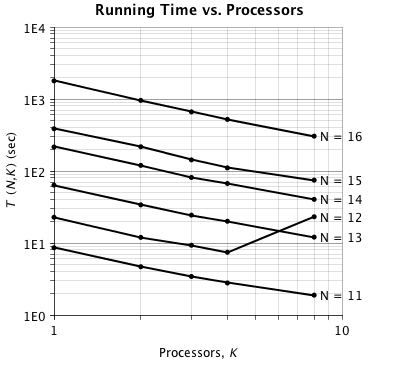
\includegraphics[scale=0.35]{./chapter_optimize/t1m_1.png}
% 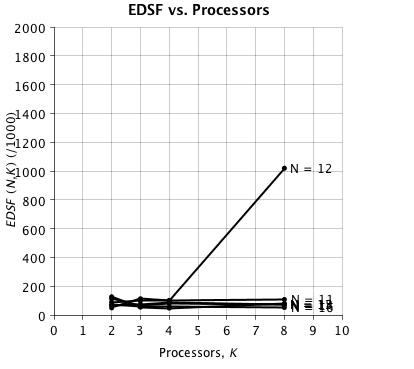
\includegraphics[scale=0.35]{./chapter_optimize/t1m_2.png}
% 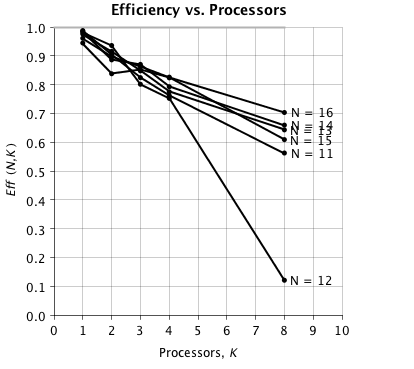
\includegraphics[scale=0.35]{./chapter_optimize/t1m_3.png}
% 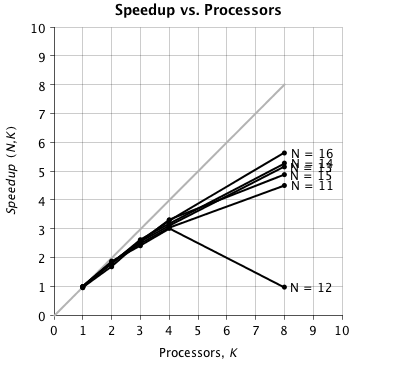
\includegraphics[scale=0.35]{./chapter_optimize/t1m_4.png}
% \caption{Speedup metrics for the parallel implementation of Boyar and Peralta's technique using tie breaker \#1 with merged $32 \times 16$ matrices.}
% \label{fig:speedup2}
% \end{center}
% \end{figure}

\begin{figure}
\begin{center}
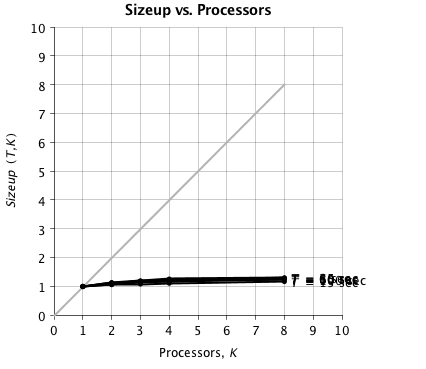
\includegraphics[scale=0.35]{./chapter_optimize/t1um_size_2.png}
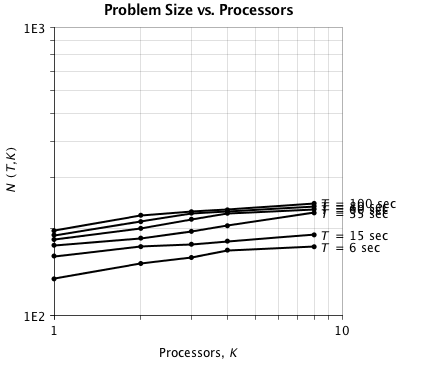
\includegraphics[scale=0.35]{./chapter_optimize/t1um_size_3.png}
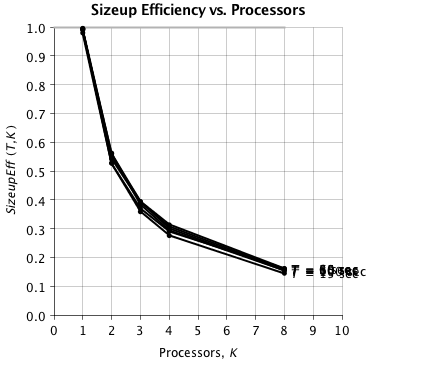
\includegraphics[scale=0.35]{./chapter_optimize/t1um_size_1.png}
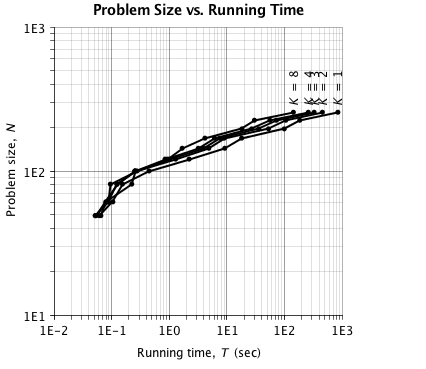
\includegraphics[scale=0.35]{./chapter_optimize/t1um_size_4.png}
\caption{Sizeup metrics for the parallel implementation of Boyar and Peralta's technique using tie breaker \#1 with merged $16 \times 16$ and unmerged matrices. This data was collected by running tests for matrices of size $7 \times 7$ to $16 \times 16$ matrices.}
\label{fig:sizeup1}
\end{center}

\begin{center}
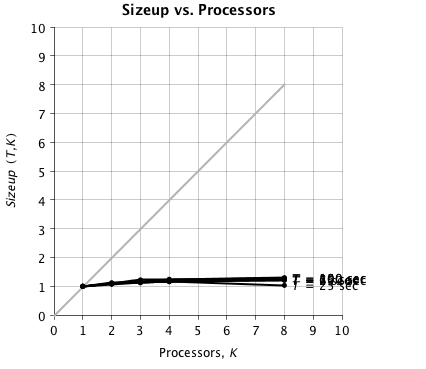
\includegraphics[scale=0.35]{./chapter_optimize/t1m_size_2.png}
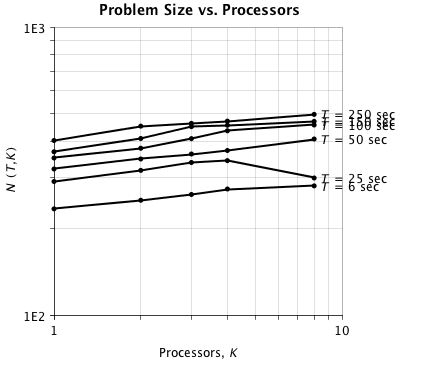
\includegraphics[scale=0.35]{./chapter_optimize/t1m_size_3.png}
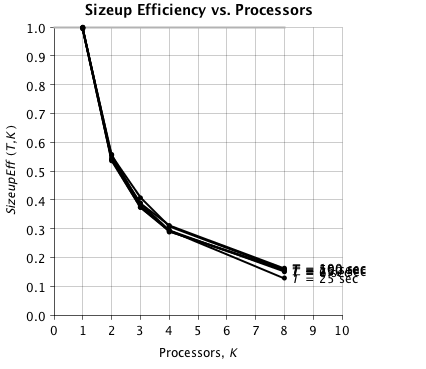
\includegraphics[scale=0.35]{./chapter_optimize/t1m_size_1.png}
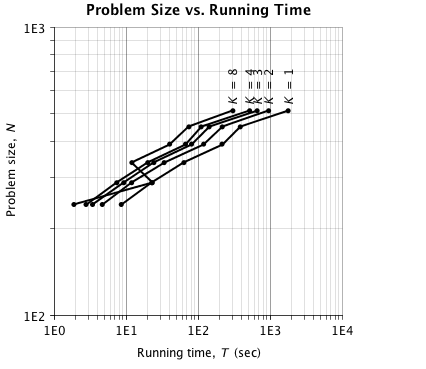
\includegraphics[scale=0.35]{./chapter_optimize/t1m_size_4.png}
\caption{Sizeup metrics for the parallel implementation of Boyar and Peralta's technique using tie breaker \#1 with merged $32 \times 16$ and unmerged matrices. This data was collected by running tests for matrices of size $22 \times 11$ to $32 \times 16$ matrices.}
\label{fig:sizeup2}
\end{center}
\end{figure}

% \begin{figure}
% \end{figure}

% \begin{figure}
% \begin{center}
% 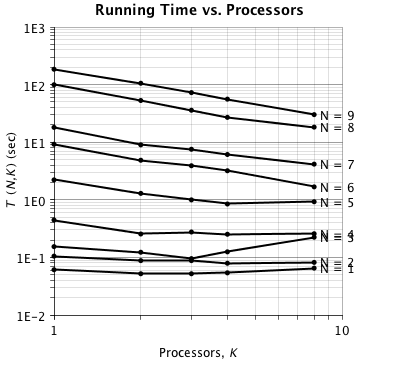
\includegraphics[scale=0.35]{./chapter_optimize/t1un_1.png}
% 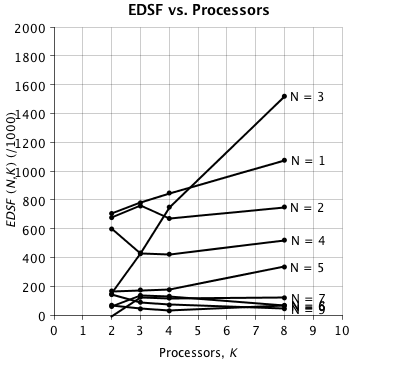
\includegraphics[scale=0.35]{./chapter_optimize/t1un_2.png}
% 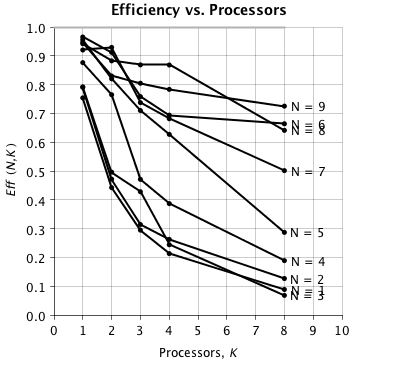
\includegraphics[scale=0.35]{./chapter_optimize/t1un_3.png}
% 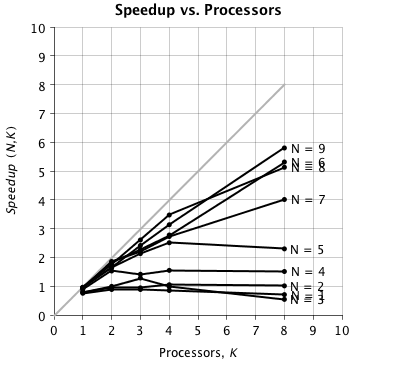
\includegraphics[scale=0.35]{./chapter_optimize/t1un_4.png}
% 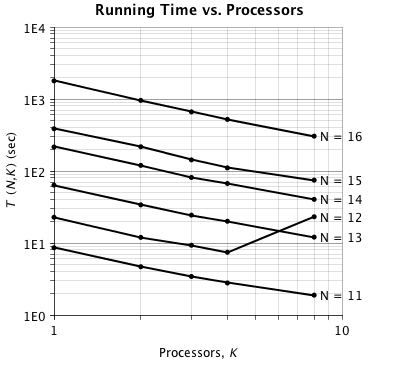
\includegraphics[scale=0.35]{./chapter_optimize/t1m_1.png}
% 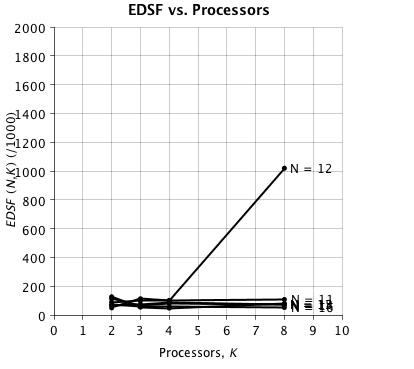
\includegraphics[scale=0.35]{./chapter_optimize/t1m_2.png}
% 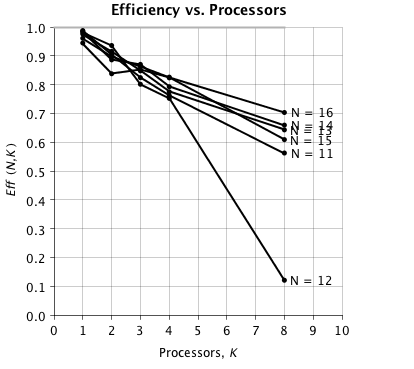
\includegraphics[scale=0.35]{./chapter_optimize/t1m_3.png}
% 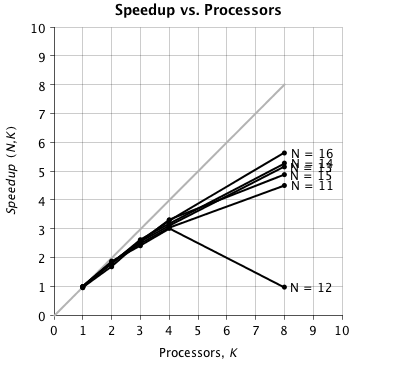
\includegraphics[scale=0.35]{./chapter_optimize/t1m_4.png}
% 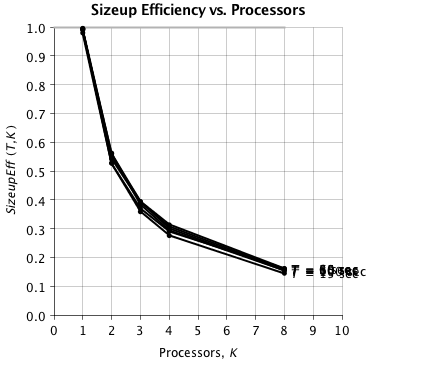
\includegraphics[scale=0.35]{./chapter_optimize/t1um_size_1.png}
% 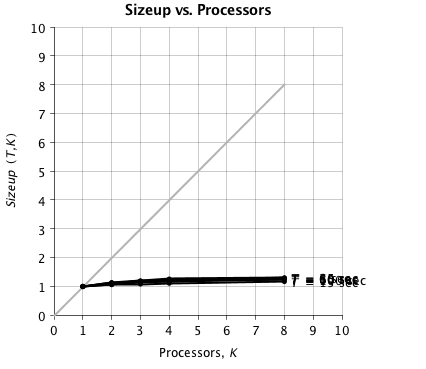
\includegraphics[scale=0.35]{./chapter_optimize/t1um_size_2.png}
% 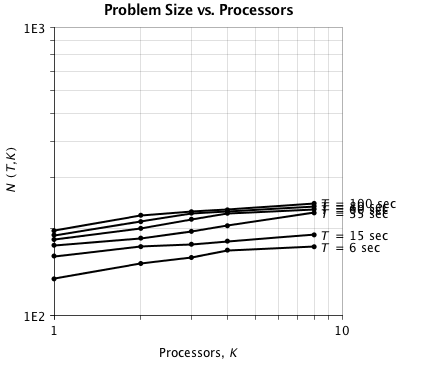
\includegraphics[scale=0.35]{./chapter_optimize/t1um_size_3.png}
% 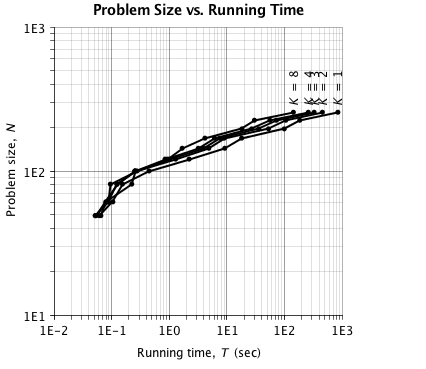
\includegraphics[scale=0.35]{./chapter_optimize/t1um_size_4.png}
% 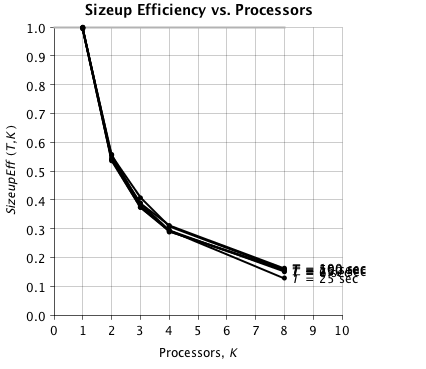
\includegraphics[scale=0.35]{./chapter_optimize/t1m_size_1.png}
% 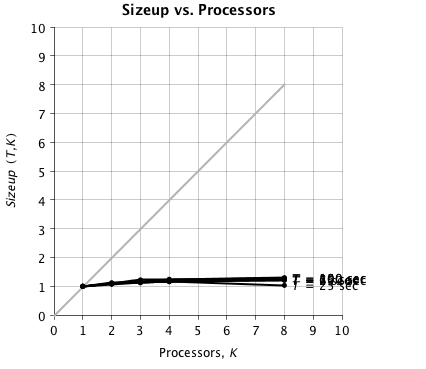
\includegraphics[scale=0.35]{./chapter_optimize/t1m_size_2.png}
% 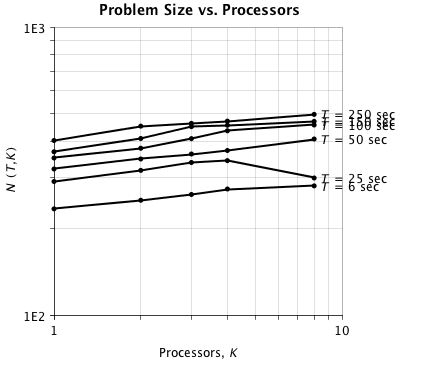
\includegraphics[scale=0.35]{./chapter_optimize/t1m_size_3.png}
% 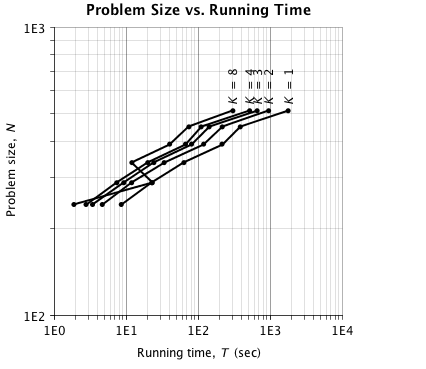
\includegraphics[scale=0.35]{./chapter_optimize/t1m_size_4.png}
% \caption{Speedup and sizeup metrics for the parallel implementation of Boyar and Peralta's technique using tie breaker \#2.}
% \label{fig:sizeup2}
% \end{center}
% \end{figure}

% \begin{figure}
% \begin{center}
% 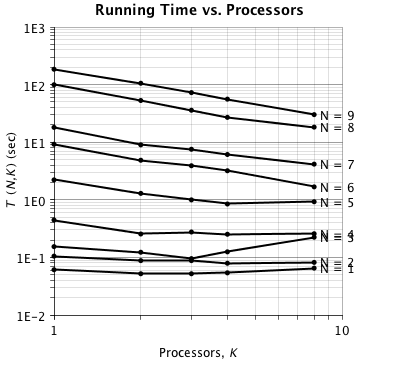
\includegraphics[scale=0.35]{./chapter_optimize/t1un_1.png}
% 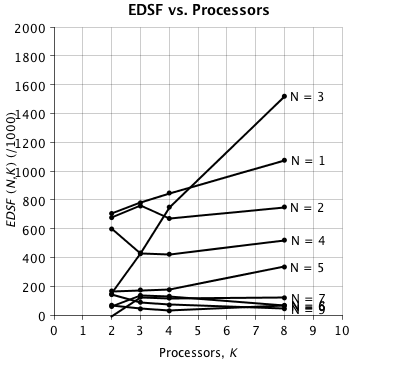
\includegraphics[scale=0.35]{./chapter_optimize/t1un_2.png}
% 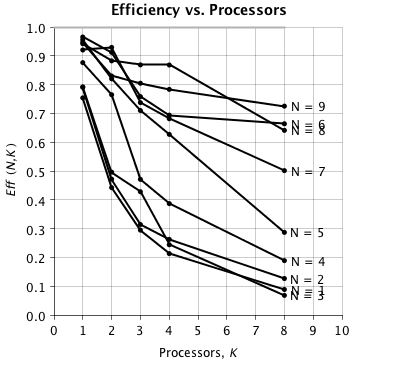
\includegraphics[scale=0.35]{./chapter_optimize/t1un_3.png}
% 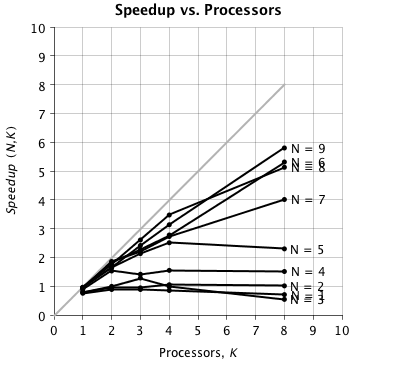
\includegraphics[scale=0.35]{./chapter_optimize/t1un_4.png}
% 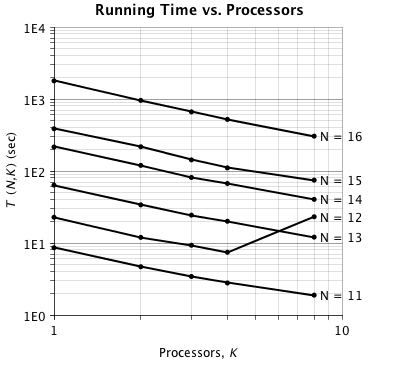
\includegraphics[scale=0.35]{./chapter_optimize/t1m_1.png}
% 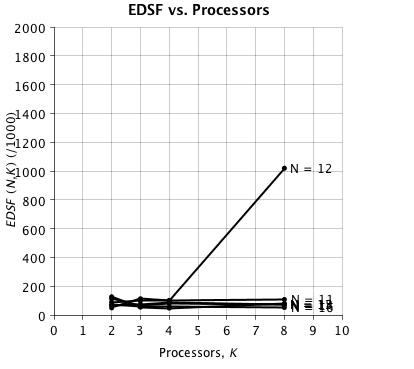
\includegraphics[scale=0.35]{./chapter_optimize/t1m_2.png}
% 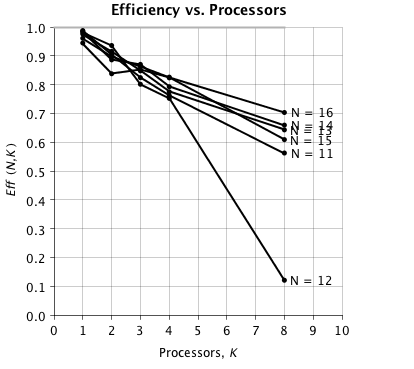
\includegraphics[scale=0.35]{./chapter_optimize/t1m_3.png}
% 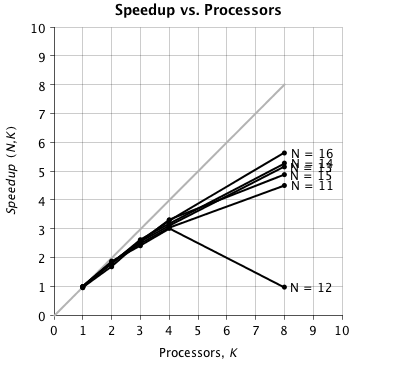
\includegraphics[scale=0.35]{./chapter_optimize/t1m_4.png}
% 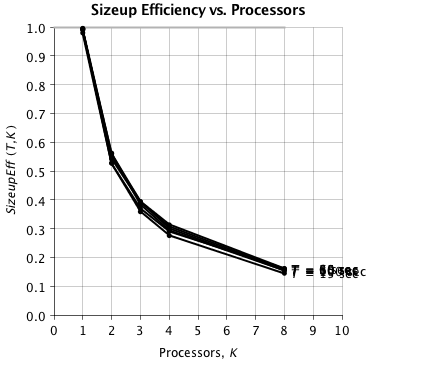
\includegraphics[scale=0.35]{./chapter_optimize/t1um_size_1.png}
% 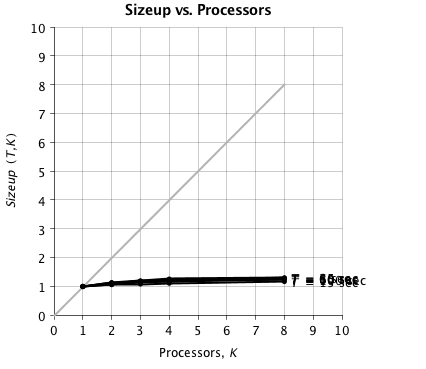
\includegraphics[scale=0.35]{./chapter_optimize/t1um_size_2.png}
% 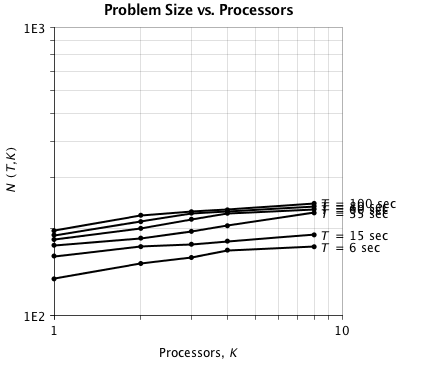
\includegraphics[scale=0.35]{./chapter_optimize/t1um_size_3.png}
% 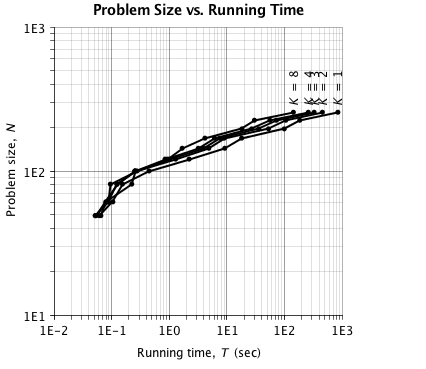
\includegraphics[scale=0.35]{./chapter_optimize/t1um_size_4.png}
% \includegraphics[scale=0.35]{./chapter_optimize/t1m_size_1.png}
% \includegraphics[scale=0.35]{./chapter_optimize/t1m_size_2.png}
% \includegraphics[scale=0.35]{./chapter_optimize/t1m_size_3.png}
% \includegraphics[scale=0.35]{./chapter_optimize/t1m_size_4.png}
% \caption{Speedup and sizeup metrics for the parallel implementation of Boyar and Peralta's technique using tie breaker \#3.}
% \label{fig:sizeup3}
% \end{center}
% \end{figure}

% \begin{figure}
% \begin{center}
% % \includegraphics[scale=0.35]{./chapter_optimize/s41.png}
% \includegraphics[scale=0.35]{./chapter_optimize/s42.png}
% \includegraphics[scale=0.35]{./chapter_optimize/s43.png}
% % \includegraphics[scale=0.35]{./chapter_optimize/s44.png}
% \caption{Speedup and sizeup metrics for the parallel implementation of Boyar and Peralta's technique using tie breaker \#4.}
% \label{fig:sizeup4}
% \end{center}
% \end{figure}
